\documentclass[12pt,]{scrartcl}
\usepackage{lmodern}
\usepackage{amssymb,amsmath}
\usepackage{ifxetex,ifluatex}
\usepackage{fixltx2e} % provides \textsubscript
\ifnum 0\ifxetex 1\fi\ifluatex 1\fi=0 % if pdftex
  \usepackage[T1]{fontenc}
  \usepackage[utf8]{inputenc}
\else % if luatex or xelatex
  \ifxetex
    \usepackage{mathspec}
  \else
    \usepackage{fontspec}
  \fi
  \defaultfontfeatures{Ligatures=TeX,Scale=MatchLowercase}
\fi
% use upquote if available, for straight quotes in verbatim environments
\IfFileExists{upquote.sty}{\usepackage{upquote}}{}
% use microtype if available
\IfFileExists{microtype.sty}{%
\usepackage{microtype}
\UseMicrotypeSet[protrusion]{basicmath} % disable protrusion for tt fonts
}{}
\usepackage[unicode=true]{hyperref}
\hypersetup{
            pdftitle={Examen DEPI -- Exemplu},
            pdfborder={0 0 0},
            breaklinks=true}
\urlstyle{same}  % don't use monospace font for urls
\usepackage{graphicx,grffile}
\makeatletter
\def\maxwidth{\ifdim\Gin@nat@width>\linewidth\linewidth\else\Gin@nat@width\fi}
\def\maxheight{\ifdim\Gin@nat@height>\textheight\textheight\else\Gin@nat@height\fi}
\makeatother
% Scale images if necessary, so that they will not overflow the page
% margins by default, and it is still possible to overwrite the defaults
% using explicit options in \includegraphics[width, height, ...]{}
\setkeys{Gin}{width=\maxwidth,height=\maxheight,keepaspectratio}
\IfFileExists{parskip.sty}{%
\usepackage{parskip}
}{% else
\setlength{\parindent}{0pt}
\setlength{\parskip}{6pt plus 2pt minus 1pt}
}
\setlength{\emergencystretch}{3em}  % prevent overfull lines
\providecommand{\tightlist}{%
  \setlength{\itemsep}{0pt}\setlength{\parskip}{0pt}}
\setcounter{secnumdepth}{0}
% Redefines (sub)paragraphs to behave more like sections
\ifx\paragraph\undefined\else
\let\oldparagraph\paragraph
\renewcommand{\paragraph}[1]{\oldparagraph{#1}\mbox{}}
\fi
\ifx\subparagraph\undefined\else
\let\oldsubparagraph\subparagraph
\renewcommand{\subparagraph}[1]{\oldsubparagraph{#1}\mbox{}}
\fi
\newcommand{\grtlessH}{\underset{{H_0}}{\overset{H_{1}}{\gtrless}}}
\renewcommand{\vec}[1]{\mathbf{#1}}

\title{Examen DEPI -- Exemplu}
\date{}

\begin{document}
\maketitle

\newcommand*{\underuparrow}[1]{\ensuremath{\underset{\uparrow}{#1}}}
\renewcommand{\vec}[1]{\mathbf{#1}}
\newcommand{\erf}{\operatorname{erf}}


Aceste este un exemplu de examen DEPI. Întrebările sunt doar în scop
ilustrativ.

\subsection{Exerciții (18p)}\label{exerciux21bii-18p}

\begin{enumerate}
\def\labelenumi{\arabic{enumi}.}
\tightlist
\item
  Fie o variabilă aleatoare \(X\) cu distribuția din figură
  \(w(x)= \begin{cases} h-\frac{h}{5}x, & x \in [0,5] \\ 0, & \textrm{în rest} \end{cases}\)

  \begin{enumerate}
  \def\labelenumii{\alph{enumii}.}
  \tightlist
  \item
    (1p) Găsiți valoarea lui \(h\) și calculați probabilitatea ca \(X\)
    să fie mai mare decât 3
  \item
    (1p) Calculați valoarea medie \(\overline{X}\)
  \item
    (2p) Găsiți expresia funcției de repartiție a lui \(x\)
  \end{enumerate}
\end{enumerate}

\begin{figure}[htbp]
\centering
\includegraphics[width=0.30000\textwidth]{fig/PDF_LinearDown.png}
\caption{Distribuția w(x)}
\end{figure}

\smallbreak

\begin{enumerate}
\def\labelenumi{\arabic{enumi}.}
\setcounter{enumi}{1}
\tightlist
\item
  Un semnal constant poate avea două valori posibile, \(-2\) (ipoteza
  \(H_0\)) sau \(4\) (ipoteza \(H_1\)). Semnalul este afectat de zgomot
  Gaussian cu distribuția \(\mathcal{N}(0, \sigma^2=4)\). La recepție se
  ia un singur eșantion \(r\). Probabilitățile celor două ipoteze sunt
  \(P(H_0) = 2/3\), \(P(H_1) = 1/3\). Decizia se ia folosind
  \textbf{criteriul plauzibilității maxime}.

  \begin{enumerate}
  \def\labelenumii{\alph{enumii}.}
  \setcounter{enumii}{1}
  \tightlist
  \item
    (1p) Scrieți expresiile matematice ale funcțiilor de plauzibilitate
    \(w(r|H_0)\) și \(w(r|H_1)\);
  \item
    (1p) Care este decizia luată, dacă eșantionul \(r\) are valoarea
    \(r = 2\)?
  \item
    (1p) Care sunt regiunile de decizie \(R_0\) și \(R_1\)?
  \item
    (2p) Calculați probabilitatea alarmei false.
  \item
    (1p) Dacă raportul de plauzibilitate
    \(\frac{w(r|H_1)}{w(r|H_0)} = 3\), care ar fi decizia luată cu
    \textbf{criteriul probabilității minime de eroare}?
  \end{enumerate}
\end{enumerate}

\smallbreak

\begin{enumerate}
\def\labelenumi{\arabic{enumi}.}
\setcounter{enumi}{2}
\tightlist
\item
  (3p) Se transmite unul dintre semnale \(s_0(t)\) sau \(s_1(t)\), iar
  la recepție se recepționează \(r(t)\). Semnalele sunt reprezentate mai
  jos. Știind că semnalele transmise sunt afectate de zgomot alb cu
  distribuție Gaussiană \(\mathcal{N}(0, \sigma^2=2)\), să se găsească
  decizia luată de receptor conform criteriului plauzibilității maxime,
  prin una dintre cele două metode:

  \begin{enumerate}
  \def\labelenumii{\roman{enumii}.}
  \tightlist
  \item
    fie prin metoda observării continue
  \item
    fie pe baza a 3 eșantioane luate la momentele \(t_1 = 0.5\),
    \(t_2 = 1.5\) și \(t_2 = 3.5\)
  \end{enumerate}
\end{enumerate}

~\includegraphics[width=0.25000\textwidth]{fig/SIG_Haar1.png} ~
\includegraphics[width=0.25000\textwidth]{fig/SIG_Haar2.png} ~
\includegraphics[width=0.25000\textwidth]{fig/SIG_Rec.png}

\smallbreak

\begin{enumerate}
\def\labelenumi{\arabic{enumi}.}
\setcounter{enumi}{3}
\tightlist
\item
  (5p) Se recepționează un semnal de forma
  \(r(t) = \underbrace{A + t + 2}_{s_\Theta(t)} + zgomot\), unde \(A\)
  este un parametru necunoscut. Zgomotul are distribuție Gaussiană
  \(\mathcal{N}(0,\sigma^2=4)\). La recepție se iau trei eșantioane, la
  momentele \(t_1 = 1, t_2 = 2, t_3 = 3\), valorile fiind \(r_1 = 6.1\),
  \(r_2 = 7.1\), \(r_3 = 8.1\). Estimați parametrul \(A\) folosind
  estimarea de plauzibilitate maximă.
\end{enumerate}

\subsection{Formule cunoscute}\label{formule-cunoscute}

\begin{itemize}
\tightlist
\item
  primitiva unei funcții Gaussiene:
  \(F(x) = \frac{1}{2}\left(1 + \erf\left(\frac{x - \mu}{\sigma \sqrt{2}}\right)\right)\)
\end{itemize}

\subsection{Teorie}\label{teorie}

\begin{enumerate}
\def\labelenumi{\arabic{enumi}.}
\item
  (1p) Fie variabila aleatoare \(X\) reprezentând numărul obținut prin
  aruncarea unui zar. Reprezentați funcția de repartiție a lui \(X\).
\item
  (2p) Enunțați teorema Wiener-Hincin.
\item
  (2p) Completați: ``Criteriul probabilității minime de eroare este
  identic cu criteriul plauzibilității maxime atunci când
  \_\_\_\_\_\_\_\_\_\_''. Justificați.
\item
  (2p) Hașurați probabilitatea condiționată de \textbf{rejecție corectă}
  (decizie corectă că semnalul nu este prezent) în cazul ipotezei
  \(H_0\), pentru criteriul Plauzibilității Maxime, pentru cele două
  funcții de plauzibilitate de mai jos. Explicați în cuvinte ce ați
  colorat.

  \begin{figure}[htbp]
  \centering
  \includegraphics[width=0.70000\textwidth]{fig/DET_DecisionRegions.png}
  \caption{}\label{id}
  \end{figure}
\item
  (3p) Fie cazul detecției unui semnal constant (0 sau A), afectat de
  \textbf{zgomot Gaussian} cu medie nulă, pe baza unui singur eșantion
  \(r\). Raportul de plauzibilitate se compară cu o valoare oarecare
  \(K\), \(\frac{w(r|H_1)}{w(r|H_0)} \grtlessH K\). Găsiți regiunile de
  decizie \(R_0\) și \(R_1\) (în funcție de \(K\)).
\item
  (1p) Dacă zgomotul care afectează un semnal \textbf{se dublează}, cum
  se modifică \textbf{raportul Semnal-Zgomot} SNR (justificați în
  cuvinte):

  \begin{enumerate}
  \def\labelenumii{\alph{enumii}.}
  \tightlist
  \item
    SNR crește
  \item
    SNR scade
  \item
    SNR rămâne constant
  \end{enumerate}
\item
  (5p) Demonstrați că minimizarea integralei
  \(I = \int_{-\infty}^\infty C(\epsilon) w(\Theta | \vec{r}) d\Theta\)
  utilizând funcția de cost pătratică
  \(C(\epsilon) = \epsilon^2 = (\hat{\Theta} - \Theta)^2\) conduce la
  formula estimatorului de Eroare Pătratică Medie Minimă (EPMM):
  \[\hat{\Theta}_{EPMM} = \int_{-\infty}^\infty \Theta w(\Theta|r) d\Theta\]
\item
  (1p) Distribuția \textbf{a posteriori} a unui parametru necunoscut
  \(\Theta\) este funcția triunghiulară de mai jos.

  \begin{enumerate}
  \def\labelenumii{\alph{enumii}.}
  \tightlist
  \item
    Care este valoarea estimatorului MAP? Explicați.
  \item
    Care este valoarea estimatorului EPMM? Explicați.
  \end{enumerate}

  \begin{figure}[htbp]
  \centering
  \includegraphics[width=0.40000\textwidth]{fig/PDF_Trig_mu5.png}
  \caption{}\label{id}
  \end{figure}
\item
  (2p) Arătați că estimarea Maximum A Posteriori este o generalizare a
  criteriului probabilității minime de eroare de la detecția semnalelor.
\end{enumerate}

\end{document}
